% Near-lossless long context — workshop / arXiv draft
% Build:  pdflatex -interaction=nonstopmode main.tex   (from papers/)
% Or:     powershell -File build_pdf.ps1
\documentclass[11pt,a4paper]{article}

\usepackage[margin=1in]{geometry}
\usepackage{times}
\usepackage{amsmath,amssymb}
\usepackage{booktabs}
\usepackage{graphicx}
\usepackage{hyperref}
\usepackage{xcolor}
\usepackage{enumitem}
\usepackage{caption}
\usepackage{microtype}
\usepackage{url}

\hypersetup{
  colorlinks=true,
  linkcolor=blue!50!black,
  citecolor=blue!50!black,
  urlcolor=blue!50!black
}

\title{\textbf{Near-Lossless Long Context under Fixed VRAM\\via Critical-Span Retention}}
\author{
  Workshop / arXiv-style draft\\
  Lab: RTX 3090 24\,GB \quad
  Primary: \texttt{Qwen/Qwen3-4B-Instruct-2507}\\
  Repo: \texttt{nearlossless-context}\quad
  Updated: 2026-07-18
}
\date{}

\begin{document}
\maketitle
\begin{abstract}
Long-context inference is limited by KV-cache memory. Training-free eviction methods shrink the cache, but it is often unclear \emph{which} tokens are necessary for near--full-KV quality, and whether online streaming fails from insufficient peak budget or from weak \textbf{query-unknown discovery}. On a multi-seed controlled retrieval suite (Qwen3-4B, RTX 3090), we show:

\begin{enumerate}[leftmargin=*,itemsep=2pt]
  \item \textbf{Structure (H1$'$).}
  Retaining critical fact tokens plus a small local radius $R^*=1$ (with attention sinks and a recent/question window) is \textbf{necessary and sufficient} for $\varepsilon\!\approx\!0$ single-fact recall: oracle \textbf{15/15}, anti-oracle \textbf{0/15}, full KV \textbf{15/15} (5 seeds $\times$ 3 depths @4k).
  \item \textbf{Discovery gap.}
  Online streaming at moderate peak fails under multi-seed hay not because the budget is too small, but because discovery is weak: attention stream@512 is \textbf{33\%}, while perfect online pin of critical$\pm R$ is \textbf{15/15} at the same peak.
  \item \textbf{Closing the gap (suite).}
  A \textbf{surface novelty detector} (within-prefix rarity + digit/ID-like cues; no final question) with \textbf{sticky pin packing} reaches $\sim$\textbf{93\%} multi-seed @4k and \textbf{100\%} ($3\times3$) through \textbf{40k} at stream@512---peak cache $\sim$\textbf{1k tokens}, flat in $L$.
  \item \textbf{Public long-doc QA (decomposition).}
  On a 60-item LongBench slice, sticky novelty lags full ($\sim$0.64$\times$ F1 at peak $\sim$1k). A \textbf{posthoc query-aware upper bound} (full prefill $\to$ compress) recovers \textbf{0.95--1.0$\times$} full F1 at final $B\in\{512,1024\}$, proving discovery \emph{can} work when the question is known. \textbf{Query-hold} streaming trades peak for quality, best $\approx$\textbf{0.92$\times$} full F1 at peak $\sim$2.5k.
\end{enumerate}

The critical-span mechanism transfers across Qwen2.5, Llama-3.2, and hybrid Gemma-4 (full layers). We do \textbf{not} claim general long-context SOTA; see Section~\ref{sec:limits}.
\end{abstract}

\section{Introduction}

KV cache memory grows with context length $L$. On a fixed workstation (here: 24\,GB), full-cache decode becomes the bottleneck long before ``the model cannot attend.'' Training-free compressors reduce tokens kept, but practice often optimizes average scores rather than \textbf{guaranteeing} the spans that encode answers---and online pipelines must score tokens \textbf{before} the user question exists.

We study \textbf{near-lossless} compression on retrieval-critical prompts: quality $Q$ should match full KV at $\varepsilon\!\approx\!0$ under a multi-seed protocol. The systems objective is
\begin{equation}
  L_\varepsilon \;=\; \max\bigl\{\, L : Q(M,L) \ge (1-\varepsilon)\,Q(\mathrm{Full},L) \,\bigr\}
\end{equation}
under \textbf{peak} cache / VRAM constraints---not only final decode size after a full prefill.

\paragraph{Claim.}
Near-lossless training-free KV compression is better understood as \textbf{retaining critical local neighborhoods} and \textbf{discovering them online before the question exists} than as uniform thinning or posthoc score ranking alone. On open long-document QA, the residual gap is largely an \textbf{online retention / peak-cache Pareto}, not a failure of query-aware scoring once the question is available.

\section{Related work}
\label{sec:related}

\paragraph{Training-free KV eviction and selection.}
A large line of work compresses the KV cache without fine-tuning by dropping low-scoring tokens. \textbf{H2O}~\cite{zhang2023h2o} keeps heavy hitters under accumulated attention; \textbf{StreamingLLM}~\cite{xiao2023streamingllm} observes attention sinks and retains initial tokens plus a sliding recent window; \textbf{Scissorhands}~\cite{liu2023scissorhands} and \textbf{TOVA}~\cite{orenzain2024tova} prune by recency/attention proxies; \textbf{SnapKV}~\cite{li2024snapkv} and pyramid-style keepers~\cite{cai2024pyramidkv} select important prefix tokens using observation-window attention, often with clustering or hierarchical budgets. These methods primarily address \emph{which scores to use when queries (or an observation window) exist}. Our contribution is complementary: multi-seed \textbf{kill tests} that isolate \emph{necessary keep sets}, an explicit \textbf{query-unknown discovery gap} for online streaming, and a lightweight surface detector + sticky packing that closes that gap on retrieval suites at flat peak cache.

\paragraph{Streaming and long-context systems.}
Chunked prefill and stream compression cap \textbf{peak} memory rather than only final decode size. We report peak cache tokens, peak VRAM, and prefill latency on a consumer GPU, in the spirit of systems-oriented long-context work rather than leaderboard-only evaluation. Hybrid architectures (sliding-window + full-attention layers; e.g.\ Gemma-4 class models) still leave full-layer KV as the dominant compressible state; we compress full layers only and keep bookkeeping for hybrid score passes.

\paragraph{Quantization.}
KV quantization (e.g.\ \textbf{KIVI}~\cite{liu2024kivi}) reduces bytes per retained token and is complementary to eviction. We use fake-int8 only for logical byte accounting in some benches; quality results use bf16 caches unless noted.

\paragraph{Benchmarks.}
Needle-in-a-haystack and multi-hop synthetic suites stress retrieval under controlled depth/seed. \textbf{LongBench}~\cite{bai2024longbench} and related public suites (RULER, InfiniteBench) stress general long-document and multi-doc QA. We use a \textbf{fixed 60-item LongBench slice} (not a full leaderboard) to separate suite success from open QA, and to measure posthoc upper bounds and peak/quality Pareto curves.

\paragraph{Positioning.}
We are not proposing a new attention kernel or claiming SnapKV-beating LongBench SOTA. The paper's contribution is a \textbf{mechanism + discovery diagnosis + workstation $L_\varepsilon$ operating point}, with honest public-data limits and a quantitative online Pareto.

\section{Methods (short)}

\paragraph{Task (suite).}
Needle-in-haystack style secrets in seeded filler; depths $\{0,0.5,1\}$; success = exact key recall (greedy decode). Stresses: NL facts, multi-needle, multi-hop, prose soft facts, multidoc.

\paragraph{H1$'$ keep set.}
sinks $\cup$ critical$\pm R$ $\cup$ recent/question window. Kill arms: full, oracle\_r1, anti\_oracle.

\paragraph{Posthoc scorer.}
\texttt{seed\_valley}: shared obs-window attention $\to$ seeds $\to$ contiguous valley + $\pm R$. Used both for suite tax tables and as the LongBench \textbf{posthoc upper bound} after full prefill.

\paragraph{Streaming.}
Chunked prefill; compress when cache $>$ budget; peak $\approx$ budget + chunk.

\paragraph{Oracle-online upper bound.}
Force-keep critical$\pm R$ whenever still in cache (perfect discovery).

\paragraph{Surface novelty (query-unknown).}
Per-token score from within-prefix rarity, first occurrence, and surface cues (digits, ID-like pieces). Expand peaks $\pm R$ into pin sets. \textbf{Sticky} registry: once discovered, pins stay until evicted; packing ranks pins by score under budget (sinks + recent reserved).

\paragraph{Query-hold (systems lever).}
Mid-stream hybrid pins under a larger \texttt{hold\_budget}, then query-aware tighten to \texttt{final\_budget} once the question is in the observation window. Peak $\approx$ hold + chunk; quality trades against peak.

\paragraph{Public LongBench slice.}
THUDM/LongBench: 20 items each of \texttt{multifieldqa\_en}, \texttt{qasper}, \texttt{hotpotqa} (60 total), contexts truncated to max 4096 tokens; token F1 vs gold + substring hit; greedy decode, max\_new$=$64.

\paragraph{Default API.}
\texttt{prefill\_auto(\ldots, mode="stream", discovery="novelty")}.\\
Use \texttt{discovery="query\_hold"} for the peak/quality Pareto path.

\section{Results}

\subsection{Figure 1 --- Story in four panels}

\begin{figure}[t]
  \centering
  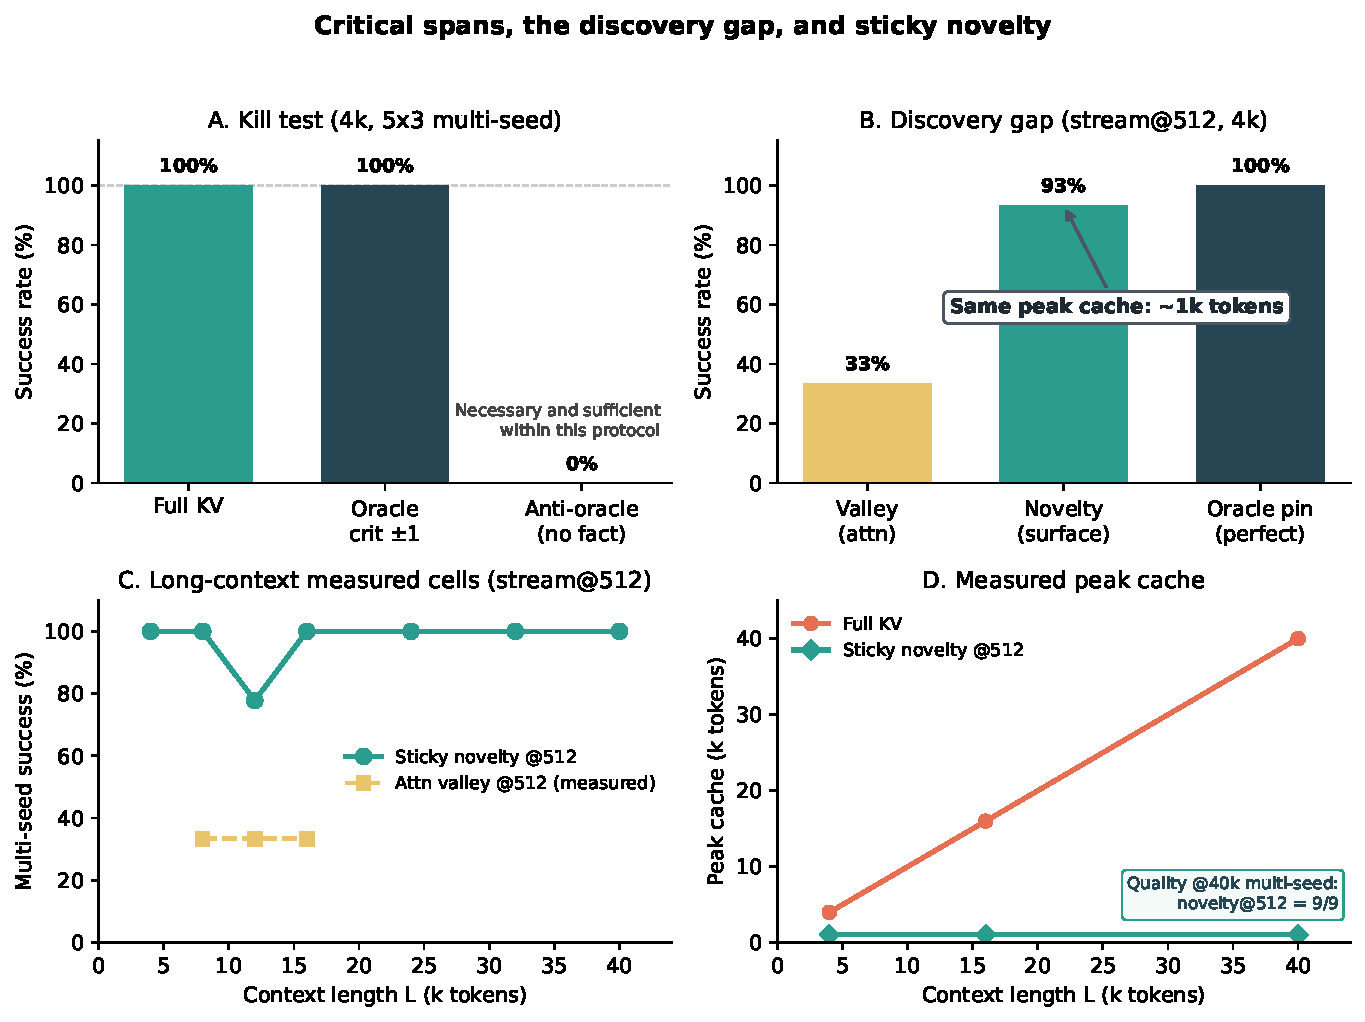
\includegraphics[width=\textwidth]{figures/fig1_story.pdf}
  \caption{\textbf{Story figure.}
  \textbf{(A)}~H1$'$ kill test @4k multi-seed ($5\times3$): full and oracle crit$\pm1$ both 15/15; anti-oracle 0/15.
  \textbf{(B)}~Discovery gap at stream@512: valley 33\%, surface novelty 93\%, oracle pin 100\%.
  \textbf{(C)}~Long-$L$ multi-seed success: sticky novelty@512 holds 9/9 through 40k; valley@512 stays end-only ($\sim$33\%).
  \textbf{(D)}~Peak cache tokens stay flat ($\sim$1k) under sticky novelty stream@512 while full KV grows with $L$.}
  \label{fig:story}
\end{figure}

\paragraph{A. H1$'$ kill (4k, $5\times3$ multi-seed).}
Full and oracle crit$\pm1$ both \textbf{15/15}; anti-oracle \textbf{0/15}. Bare critical tokens without radius often corrupt trailing digits (H1 needs local context); $R^*=1$ restores $\varepsilon\!\approx\!0$. Mean $|\mathrm{oracle}| \approx$ \textbf{149} tokens vs full $\sim$4k.

\paragraph{B. Discovery gap (stream@512).}
Attention valley \textbf{33\%}; surface novelty \textbf{93\%} (14/15); oracle pin \textbf{100\%}. Peak budget is in the same class ($\sim$1k with chunk). Failures of valley at 512 are \textbf{detector} failures, not ``stream cannot work.''

\paragraph{C. Long $L$ multi-seed ($3\times3$).}
Sticky novelty@512 is \textbf{9/9} at 16k, 24k, 32k, and \textbf{40k}. Non-sticky novelty degraded at 24k ($\sim$6/9) via re-rank thrash; sticky packing fixed it. Valley@512 remains end-depth-only ($\sim$33\%) under multi-seed hay as $L$ grows.

\paragraph{D. Peak cache.}
Full KV scales with $L$; sticky novelty stream@512 stays $\sim$\textbf{1k} tokens. Prior valley operating points often used $\sim$1.5--2k peak for long $L$.

\subsection{Scorer tax (posthoc, question known)}

\begin{table}[h]
\centering
\caption{Posthoc budget tax vs oracle keep set (4k multi-seed).}
\label{tab:tax}
\begin{tabular}{@{}lcc@{}}
\toprule
Method & All-cell $B_{\min}$ & Tax vs mean $|\mathrm{oracle}|$ \\
\midrule
oracle\_r1 & $\sim$149 & $1.0\times$ \\
seed\_valley & \textbf{192} & $\sim$\textbf{1.24}$\times$ global / $\sim$\textbf{1.16}$\times$ mean \\
\bottomrule
\end{tabular}
\end{table}

Posthoc is near-oracle-tight; \textbf{stream is not}, until discovery improves.

\subsection{Stress and transfer (summary)}

\begin{table}[h]
\centering
\caption{Stress suite and cross-model transfer (summary).}
\label{tab:transfer}
\begin{tabular}{@{}lp{0.55\textwidth}@{}}
\toprule
Check & Result \\
\midrule
NL facts (names/places) sticky novelty@512 & \textbf{15/15} multi-seed \\
Code needles sticky & \textbf{15/15} \\
Adversarial ID-like filler (pre-sticky) & novelty \textbf{100\%} vs valley \textbf{33\%} \\
Multi-needle recall\_all @512 & novelty \textbf{5/5} (\texttt{max\_new}$\ge$96); valley \textbf{0/5} \\
2-hop (Alice$\to$id$\to$password) @512 & novelty \textbf{5/5}; valley \textbf{1/5} (needs @1024 for 5/5) \\
3-hop + distractors @512 & novelty \textbf{5/5}; valley \textbf{0/5} (needs @1024 for 5/5) \\
Prose soft fact (no digits) @512 & novelty \textbf{15/15}; valley 53\% \\
Multidoc (6 titled docs) @512 & novelty \textbf{15/15}; valley/oracle\_pin \textbf{5/15} \\
External-style mixed QA (10$\times$$\sim$4k) & novelty \textbf{10/10} hits (= full); valley \textbf{0/10} \\
Gemma-4 E4B hybrid novelty@512 & multi-seed \textbf{9/9} @4k (valley needs $\sim$1024) \\
Qwen2.5 / Llama-3.2 & H1 holds; family-specific posthoc floors \\
\bottomrule
\end{tabular}
\end{table}

\subsection{Public LongBench decomposition}
\label{sec:longbench}

Synthetic suite success does not automatically transfer to open long-document QA. On the fixed 60-item slice (same items for all arms), sticky novelty stream@512 is only slightly above attention streaming and far below full (Table~\ref{tab:lb-posthoc}). A posthoc query-aware upper bound---full prefill, then \texttt{seed\_valley} compress with the question in the observation window---recovers \textbf{0.95$\times$} full mean F1 at final $B{=}512$ and $\sim$\textbf{1.0$\times$} at 1024/2048. Peak remains full $L$ for posthoc; the point is diagnostic: \textbf{query-aware scoring can keep answer-bearing tokens} when allowed to see the full prefix and the question.

\begin{table}[t]
\centering
\caption{LongBench slice (60 items @4k truncate): posthoc upper bound vs full.
Peak for posthoc is full $L$ (not a free systems win).}
\label{tab:lb-posthoc}
\small
\begin{tabular}{@{}lcccc@{}}
\toprule
Arm & Mean F1 & Substr hit & Peak & F1 / full \\
\midrule
full & \textbf{0.282} & 25\% & $=L$ & $1.00\times$ \\
posthoc@512 & 0.267 & 27\% & $=L$ & \textbf{0.95$\times$} \\
posthoc@1024 & 0.284 & 28\% & $=L$ & $\sim$1.01$\times$ \\
posthoc@2048 & 0.285 & 27\% & $=L$ & $\sim$1.01$\times$ \\
\bottomrule
\end{tabular}
\end{table}

Online paths must drop tokens before the question exists. Table~\ref{tab:lb-pareto} reports a \textbf{query-hold Pareto}: larger mid-stream hold improves recovery after query-aware tighten; final budget 1024 consistently beats 512 at fixed hold. Best measured online point: hold $2048\to$ final $1024$ $\approx$ \textbf{0.92$\times$} full F1 at mean peak $\sim$2.5k tokens---between novelty@1k (0.64$\times$) and full@$L$.

\begin{table}[t]
\centering
\caption{LongBench slice: online quality vs peak cache (query-hold Pareto).}
\label{tab:lb-pareto}
\small
\begin{tabular}{@{}lcccc@{}}
\toprule
Arm & Mean F1 & Hit & Mean peak & F1 / full \\
\midrule
novelty@512 & 0.179 & 10\% & 1024 & $0.64\times$ \\
query\_hold h1024$\to$f512 & 0.199 & 18\% & 1536 & $0.70\times$ \\
query\_hold h1024$\to$f1024 & 0.231 & 22\% & 1536 & $0.82\times$ \\
query\_hold h2048$\to$f512 & 0.212 & 17\% & $\sim$2531 & $0.75\times$ \\
\textbf{query\_hold h2048$\to$f1024} & \textbf{0.260} & 22\% & $\sim$\textbf{2531} & \textbf{0.92$\times$} \\
query\_hold h4096$\to$f1024 & 0.249 & 28\% & $\sim$3876 & $0.88\times$ \\
\bottomrule
\end{tabular}
\end{table}

\paragraph{Interpretation.}
Open long-doc QA on this slice is not primarily ``seed\_valley cannot find answers when query-aware.'' It is an \textbf{online retention} problem. Systems claims should be stated as a peak/quality curve, not as free near-full quality at peak$\sim$1k outside retrieval suites.

\subsection{Systems resources (peak VRAM / latency)}

Mid-depth needle, seed 0. Novelty stream@512 keeps peak VRAM and decode KV essentially flat:

\begin{table}[h]
\centering
\caption{Peak resources: full chunked prefill vs sticky novelty stream@512.}
\label{tab:resources}
\small
\begin{tabular}{@{}rrrrrr@{}}
\toprule
$L$ & full VRAM & nov.\ VRAM & full KV & nov.\ KV & nov.\ prefill \\
\midrule
4k & 8.5\,GB & \textbf{8.3\,GB} & 569\,MB & \textbf{72\,MB} & 1.6\,s \\
16k & 10.6\,GB & \textbf{8.3\,GB} & 2296\,MB & \textbf{72\,MB} & 5.9\,s \\
40k & 14.5\,GB & \textbf{8.3\,GB} & 5754\,MB & \textbf{72\,MB} & 17.6\,s \\
\bottomrule
\end{tabular}
\end{table}

Peak cache under novelty stays $\sim$1024 tokens at all three lengths.

\section{Adaptive policy (systems)}

\texttt{prefill\_auto} applies $L$-based budgets + per-model floors. With default \texttt{discovery="novelty"}, single-needle stream@\textbf{512} is the measured multi-seed operating point through \textbf{40k}. Attn-only discovery still needs larger floors ($\sim$1536 multi-seed @4k). Hybrid Gemma: compress \textbf{full} layers only; sliding layers keep absolute prefix bookkeeping for score-pass.

\section{Limitations and what we do \emph{not} claim}
\label{sec:limits}

\subsection{What we claim}

\begin{itemize}[leftmargin=*,itemsep=2pt]
  \item On this \textbf{controlled multi-seed retrieval suite}, critical$\pm R^*$ is necessary/sufficient for $\varepsilon\!\approx\!0$ single-fact recall.
  \item Stream failures at moderate budget are primarily a \textbf{query-unknown discovery} problem (oracle-online upper bound).
  \item Sticky surface novelty \textbf{closes most of that gap} through \textbf{40k} multi-seed at peak cache $\sim$1k on the primary model, with transfer smoke to other small instruct models including hybrid Gemma-4.
  \item On public LongBench, \textbf{posthoc query-aware compression $\approx$ full} at final $B{=}512$ (peak=$L$), while online novelty lags; \textbf{query\_hold} recovers a measured Pareto (best $\sim$0.92$\times$ full F1 at peak $\sim$2.5k).
\end{itemize}

\subsection{What we do \emph{not} claim}

\begin{table}[h]
\centering
\caption{Scope boundaries (honest).}
\label{tab:noclaim}
\small
\begin{tabular}{@{}p{0.32\textwidth}p{0.58\textwidth}@{}}
\toprule
\textbf{Not claimed} & \textbf{Why} \\
\midrule
General long-context SOTA &
  No full RULER / LongBench / InfiniteBench leaderboard evaluation. \\
All task types &
  Primary suite is retrieval / needle-class (+ multi-needle, hops, prose, multidoc stress). Full reasoning chains, code repos, and full LongBench/RULER leaderboards untested. \\
Oracle-tight online budgets for free &
  Sticky novelty $\approx$ oracle quality on this suite at@512, but multi-secret packing ($\sim$80\% multi3) and suite-alignment remain. \\
Production memory stack &
  Fake-int8 is logical accounting only; no fused kernels or serving productization. \\
Novelty as universal ``importance'' &
  Exploits surface distinctness vs repetitive filler; ID-like filler / filler-like secrets can still confuse discovery. \\
Large models / training-free SOTA &
  Primary evidence is $\sim$3--4B instruct models on one GPU class. \\
Statistical finality &
  Multi-seed $N$ modest ($5\times3$ @4k; $3\times3$ long-$L$). Lab-grade, not a large meta-analysis. \\
$\varepsilon\!=\!0$ beyond measured envelope &
  Sticky multi-seed measured through \textbf{40k}; longer $L$ is extrapolation. \\
Peak VRAM $=$ final decode KV &
  Streaming caps \textbf{peak cache tokens}; weights and activations still dominate total VRAM. \\
\bottomrule
\end{tabular}
\end{table}

\subsection{Threats to validity}

\begin{itemize}[leftmargin=*,itemsep=2pt]
  \item \textbf{Greedy decode} and chat templates may interact with exact-match scoring.
  \item \textbf{Filler distribution} is synthetic; natural corpora may change novelty baselines.
  \item \textbf{Hybrid models:} only full layers are compressed; sliding-window behavior is infrastructure-sensitive.
  \item \textbf{Selection bias toward positive arms:} we iterated methods until discovery worked; negative results (scored capsules alone, non-sticky long-$L$) are reported but the path is research-in-the-loop.
\end{itemize}

\section{Conclusion}

Near-lossless training-free KV compression on retrieval tasks is structured by \textbf{critical local neighborhoods}. When the question is known, a simple attention valley scorer approximates the oracle keep set with small tax---and on a public LongBench slice, posthoc query-aware compression reaches $\sim$full quality at final $B{=}512$. When the question is \textbf{not} known---as in online streaming---the binding constraint is \textbf{discovery}/retention before the query. Sticky surface novelty is a lightweight query-unknown detector that, on our multi-seed suite, restores high success through \textbf{40k} context at a \textbf{flat $\sim$1k-token peak cache}. On open long-doc QA, quality becomes a \textbf{Pareto} in peak cache (query-hold $\sim$0.92$\times$ full F1 at $\sim$2.5k peak). Honest next steps are better mid-stream pins and multi-entity packing---not larger single-needle grids alone.

\section*{Reproducibility}

\begin{verbatim}
# Multi-seed H1 + scorer tax
python experiments/bench_paper_rigor.py --seeds 0,1,2,3,4 --ctx 4096

# Discovery gap / novelty
python experiments/bench_capsules.py --novelty --oracle-online \
  --skip-capsules --budgets 512
python experiments/bench_novelty_stress.py
python experiments/bench_novelty_longL.py \
  --ctx 16384,24576,32768,40960 --arms novelty --budgets 512

# LongBench posthoc UB + query_hold Pareto (60 items)
python experiments/bench_external_slice.py --source longbench --n 60 \
  --arms full,posthoc --budgets 512,1024,2048
python experiments/bench_external_slice.py --source longbench --n 60 \
  --arms full,novelty,query_hold --budgets 512 \
  --hold-budgets 1024,2048,4096 --final-budgets 512,1024

# Figure + transfer
python experiments/plot_paper_figures.py
python experiments/bench_transfer.py --model google/gemma-4-E4B-it
\end{verbatim}

\noindent
\textbf{Primary model:} \texttt{Qwen/Qwen3-4B-Instruct-2507}, transformers, CUDA bf16, RTX 3090.\\
\textbf{Artifact index:} \texttt{results/FINDINGS.md}.\\
\textbf{Markdown twin:} \texttt{papers/PAPER\_DRAFT.md}.\\
\textbf{Build PDF:} from \texttt{papers/}, run \texttt{powershell -File build\_pdf.ps1}.

\begin{thebibliography}{99}

\bibitem{zhang2023h2o}
Z.~Zhang et~al.
\newblock H$_2$O: Heavy-Hitter Oracle for Efficient Generative Inference of Large Language Models.
\newblock \emph{NeurIPS}, 2023.

\bibitem{xiao2023streamingllm}
G.~Xiao et~al.
\newblock Efficient Streaming Language Models with Attention Sinks.
\newblock \emph{ICLR}, 2024.

\bibitem{liu2023scissorhands}
Z.~Liu et~al.
\newblock Scissorhands: Exploiting the Persistence of Importance Hypothesis for LLM KV Cache Compression at Test Time.
\newblock \emph{NeurIPS}, 2023.

\bibitem{orenzain2024tova}
M.~Oren et~al.
\newblock Transformers are Multi-State RNNs (TOVA).
\newblock \emph{arXiv:2401.06104}, 2024.

\bibitem{li2024snapkv}
Y.~Li et~al.
\newblock SnapKV: LLM Knows What You are Looking for Before Generation.
\newblock \emph{NeurIPS}, 2024.

\bibitem{cai2024pyramidkv}
Z.~Cai et~al.
\newblock PyramidKV: Dynamic KV Cache Compression based on Pyramidal Information Funneling.
\newblock \emph{arXiv:2406.02069}, 2024.

\bibitem{liu2024kivi}
Z.~Liu et~al.
\newblock KIVI: A Tuning-Free Asymmetric 2bit Quantization for KV Cache.
\newblock \emph{ICML}, 2024.

\bibitem{bai2024longbench}
Y.~Bai et~al.
\newblock LongBench: A Bilingual, Multitask Benchmark for Long Context Understanding.
\newblock \emph{ACL}, 2024.

\end{thebibliography}

\end{document}
